\documentclass[12pt]{article}
\usepackage{fullpage,graphicx,amsmath,amsfonts,forest,listings,xcolor}
\usepackage[hidelinks]{hyperref}
\usepackage[small,bf]{caption}

\definecolor{bgcolor}{rgb}{0.95,0.95,0.95}
\lstdefinestyle{mystyle}{
basicstyle=\footnotesize\ttfamily,
backgroundcolor=\color{bgcolor},
keywordstyle=\color{violet},
stringstyle=\color{red},
showstringspaces=false,
numbers=left,
frame=line
}
\lstset{
style=mystyle,
breaklines=true,
postbreak=\mbox{\textcolor{red}{$\hookrightarrow$}\space}
}

\input defs.tex

\bibliographystyle{alpha}

\title{
Programming Assignments 2: Java Parser \\
\large CSE360, Design and Implementation of Compiler
}
\author{
Shao-Hsuan Chu \\
Instructor: Ye-In Chang \\
Teaching Assistant: Sheng-Hsin Chiang \\
\\
National Sun Yat-sen University
}

\begin{document}
\maketitle

\tableofcontents
\newpage

\section{Introduction}
In this assignment, we're required to implement a syntactic parser for Java programming language in Lex \& Yacc. The parser need to have three main features below.

\begin{itemize}
    \item A scanner to correctly extract tokens from the raw input and pass them onto the next stage. It also has to identify the redundant characters if they cannot be recognized as any token.
    \item A parser to examine the syntactic structure based on a pre-defined Java grammar. Upon encountering an error, it needs to be able to recover and keep parsing the rest of the input source file. An expressive error message is also preferred.
    \item A simple semantic check for redefinitions in the same scope and unused variables.
\end{itemize}

\section{File structure}

\begin{forest}
for tree={
font=\ttfamily,
grow'=0,
child anchor=west,
parent anchor=south,
anchor=west,
calign=first,
edge path={
\noexpand\path [draw, \forestoption{edge}]
(!u.south west) +(7.5pt,0) |- node[fill,inner sep=1.25pt] {} (.child anchor)\forestoption{edge label};
},
before typesetting nodes={
if n=1
{insert before={[,phantom]}}
{}
},
fit=band,
before computing xy={l=50pt},
}
[.
    [README.pdf]
    [TestingFiles
	[test1-6.java]
    ]
    [src
	[B073040018.l]
	[B073040018.y]
	[Makefile]
	[SymbleTable
	    [SymbolTable.c]
	    [SymbolTable.h]
	]
	[utils
	    [ListOptionals.sh]
	    [ListTokens.sh]
	]
    ]
]
\end{forest}

\begin{itemize}
    \item \texttt{README.pdf}: This file
    \item \texttt{TestFiles}
    \begin{itemize}
	\item \texttt{test1-6.java}: six testing files
    \end{itemize}
    \item \texttt{src}: source code
    \begin{itemize}
	\item \texttt{B073040018.l}: Lex code
	\item \texttt{B073040018.y}: Lex code
	\item \texttt{Makefile}: Compile Lex, Yacc and C source code
	\item \texttt{SymbolTable}: Symbol table header and implementation using hash table
	\item \texttt{utils}: Utilities
	\begin{itemize}
	    \item \texttt{ListOptionals.sh}: Take Lex source file and extract the tokens after the keyword \texttt{return} and removes the duplicates.
	    \item \texttt{ListTokens.sh}: Take Yacc source file and extract all of the optionals then generates the rules for them.
	\end{itemize}
    \end{itemize}
\end{itemize}

\section{Environment}
\subsection{Operating systems}
\begin{itemize}
    \item macOS 11.4
    \item Ubuntu 18.04.5 LST
\end{itemize}
\subsection{Lex compiler}
\begin{itemize}
    \item flex 2.5.35 Apple(flex-32)
    \item flex 2.6.4
\end{itemize}
\subsection{Yacc compiler}
\begin{itemize}
    \item bison (GNU Bison) 2.3
    \item bison (GNU Bison) 3.0.4
\end{itemize}

\section{Usage}
\subsection{Build}
To build the \texttt{JavaParser} from source, use \texttt{make}.

\begin{lstlisting}[language=sh]
cd src
make [DEBUG=<level>]
\end{lstlisting}

where you can set the optional flag \texttt{DEBUG} to a desired level. If the flag is not provided, then it defaults to level \texttt{0}.
\subsection{Debug level}
The available levels include:

\begin{itemize}
    \item \texttt{Level 0}: Print the errors and warnings only.
    \item \texttt{Level 1}: Print the original source code and errors/warnings in the context.
    \item \texttt{Level 2}: Same as above but this one also prints the symbol table.
    \item \texttt{Level 3}: In addition to above, this also prints the entire parsing process. This sets \texttt{yydebug} to \texttt{1} in the Yacc source file and generate \texttt{y.output}, which contains all of the states and rules.
\end{itemize}

\subsection{Execute}
To parse a Java source file, redirect the content into the program. The \texttt{TestingFiles} directory contains six testing files. To test a single file
\begin{lstlisting}[language=sh]
./JavaParser < ../TestingFiles/test1.java
\end{lstlisting}
to test all files altogether
\begin{lstlisting}[language=sh]
cat ../TestingFiles/* | ./JavaParser
\end{lstlisting}



\section{Implementation}
\subsection{Lexical analysis}

Despite the Java's capability of allowing Unicode characters, only ASCII characters can be accepted by the parser in this work for the sake of simplicity. In lexical analysis, the mission is to combine one or more characters in to various tokens. The tokens can be divided into three main groups which are \texttt{literals}, \texttt{keywords \& operators} and \texttt{identifier \& others}. 

\subsubsection{Literals}

There are six kinds of literals in Java. They are

\paragraph{Boolean literal.}
For the boolean literal, the accepted words can be either \texttt{true} or \texttt{false}.
\paragraph{Null literal.}
For the null literal, it just accepts \texttt{null}.
\paragraph{Character literal.}
For the character literal, the content must be included in two single quotes and it accept any character except \texttt{single quote}, \texttt{new line character}, and \texttt{backslash}. However, the escape sequence is also accepted by the content. See the following Lex source code.
\lstinputlisting[linerange={23-24}]{../src/B073040018.l}
\paragraph{String literal.}
For the string literal, the content must be included in two double quotes and it accept any characters except \texttt{double quotes}, \texttt{new line characters}, and \texttt{backslashes}. However, the escape sequence is also accepted by the content. See the following Lex source code.
\lstinputlisting[linerange={25-25}]{../src/B073040018.l}
\paragraph{Integer literal.}
The integer literal can be further decomposed into \texttt{decimal}, \texttt{hexadecimal} and \texttt{octal} integer literals with a shared optional postfix \texttt{l} or \texttt{L}. See the following Lex source code.
\lstinputlisting[linerange={27-31}]{../src/B073040018.l}
\paragraph{Floating-point literal.}
The floating-point literal accepts the integer literal plus \texttt{decimal point} and \texttt{scientific notation} with an optional postfix \texttt{f} or \texttt{F} for single-precision floating-point and \texttt{d} or \texttt{D} for the double-precision one.
\lstinputlisting[linerange={33-33}]{../src/B073040018.l}

\subsubsection{Keywords \& Operators}
\paragraph{Keywords}
The keywords in Java is reserved. Defining them before the identifier prevents the word from being matched with the identifier token. Here's a list of keywords in the original Java. Noted that \texttt{const} and \texttt{goto} are keywords but never used in Java, hence none of the productions in the next stage use them. Consequently, we don't have to pass them as tokens onto the next stage of parsing.
\begin{lstlisting}[language=Java]
abstract boolean break byte case catch char class const continue default 
do double else extends final finally float for goto if implements import 
instanceof int interface long native new package private protected public
return short static super switch synchronized this throw throws transient
try void volatile while
\end{lstlisting}
\paragraph{Operators}
We also need to capture the operators one by one and pass them as tokens onto the next stage. Here's a list of operators in Java.
\begin{lstlisting}[language=Java]
= *= /= %= += -= <<= >>= >>>= &= ^= |= << >> >>> == != <= >= < > && || ! ++ -- & | ^ ~ * / % + - ? : . { } [ ] ( ) , ;
\end{lstlisting}

\subsubsection{Identifier \& Others}
\paragraph{Identifier}
The identifier in Java can start with any Unicode characters except digits and some symbols. However, as mentioned above, only ASCII characters are allowed in this work. As the regular expression goes
\lstinputlisting[linerange={35-35}]{../src/B073040018.l}

\paragraph{Others}
Other tokens include \texttt{space}, \texttt{new line character} and \texttt{comment}. There are recognized so they won't be redundant characters, but they won't be passed onto the next stage, either. The space includes single space characters and tabular characters while the comment allows both C-style (/* */) and C++-style (//) comments. See the regular expressions below.

\lstinputlisting[linerange={36-37}]{../src/B073040018.l}

\subsection{Syntax analysis}

\section{Screenshots}

\begin{figure}
\begin{center}
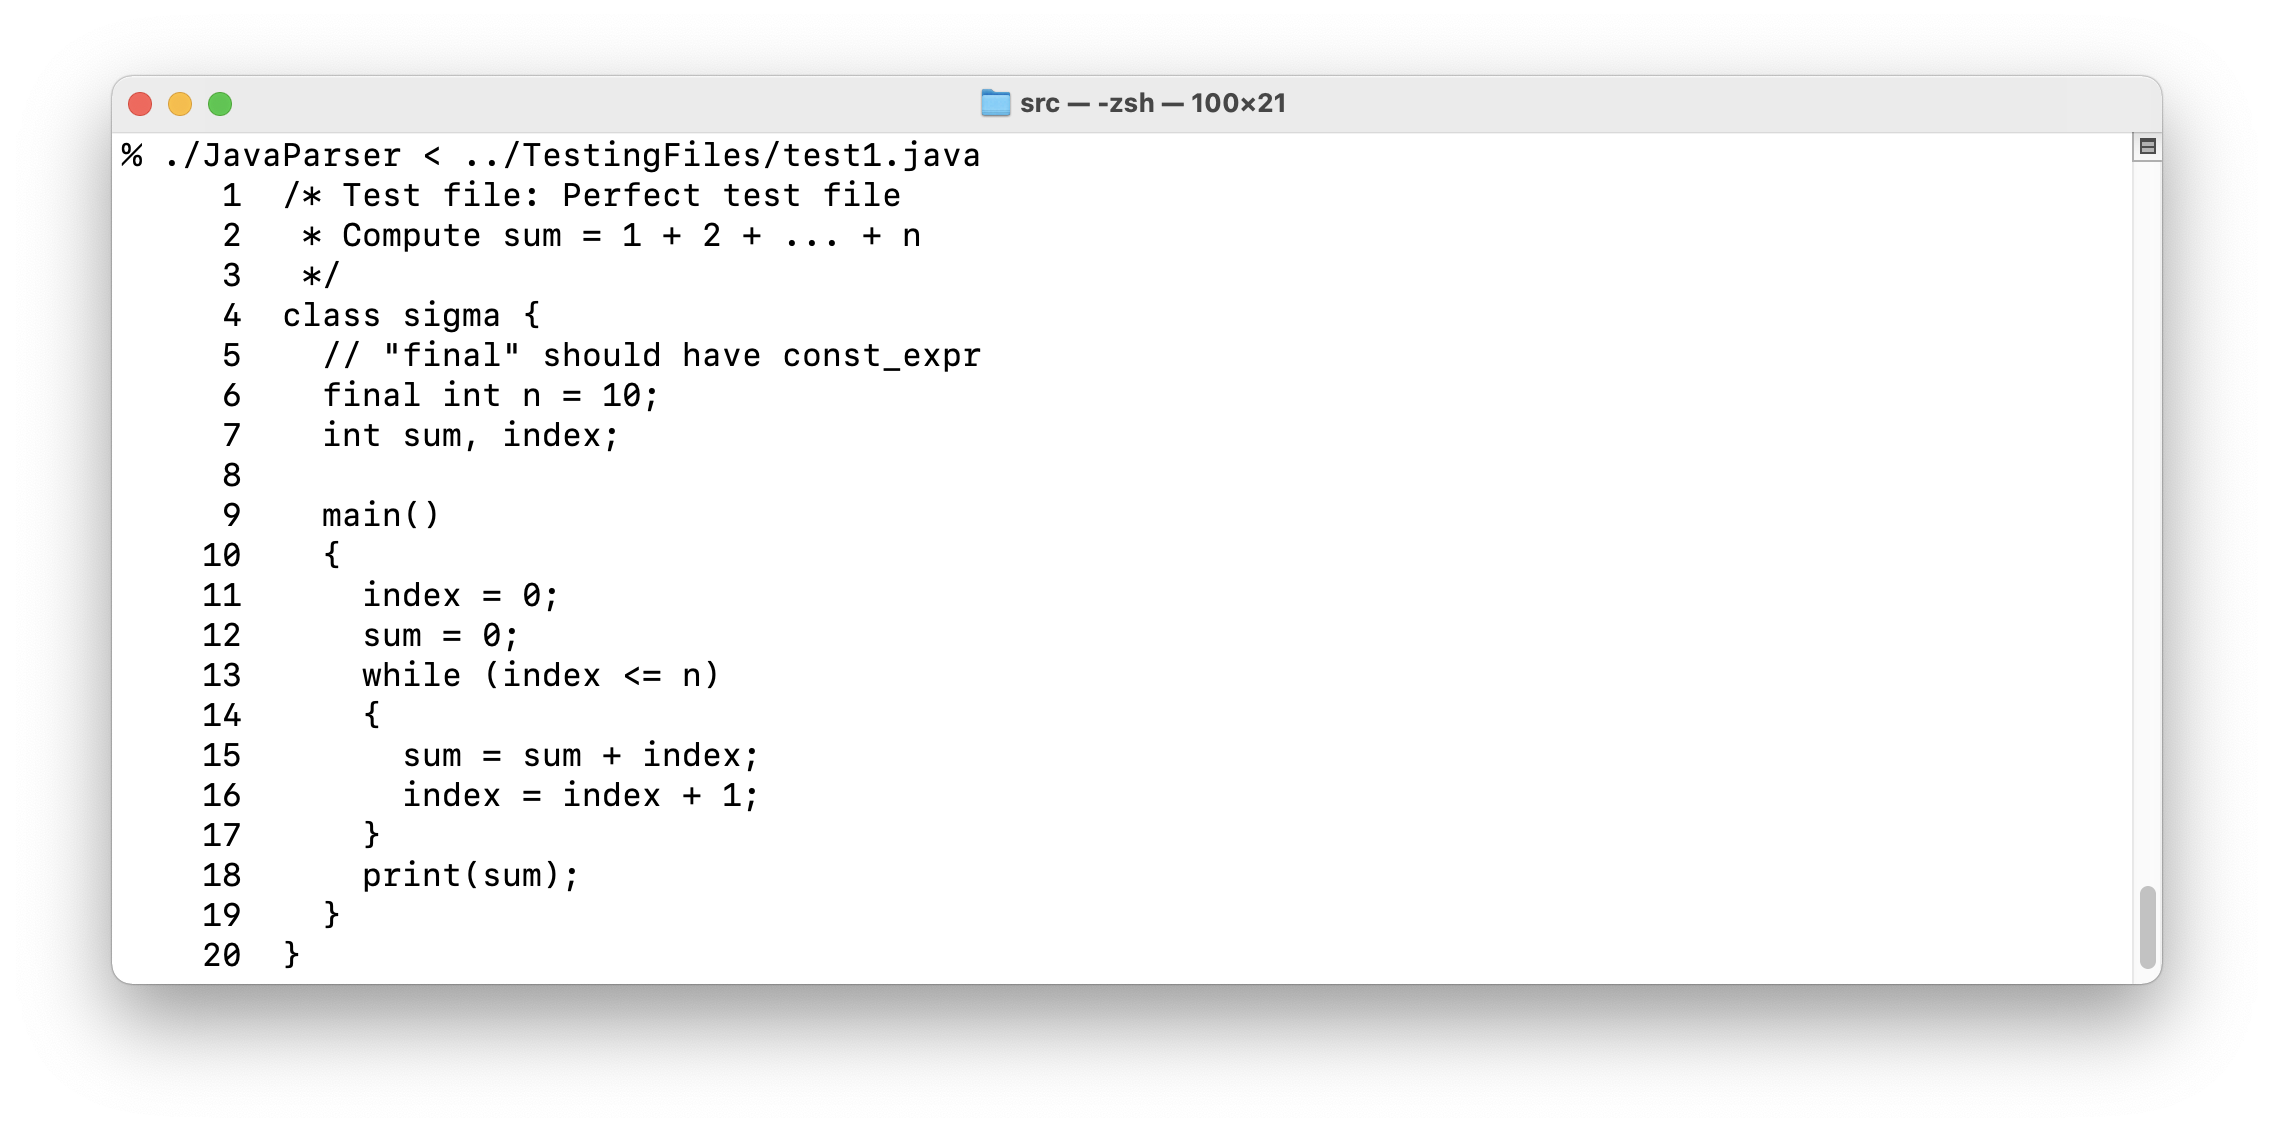
\includegraphics[width=0.9\textwidth]{Screenshots/test1}
\end{center}
\caption{The output of parsing \texttt{test1.java} with \texttt{DEBUG=1}}
\label{test1}
\end{figure}
\begin{figure}
\begin{center}
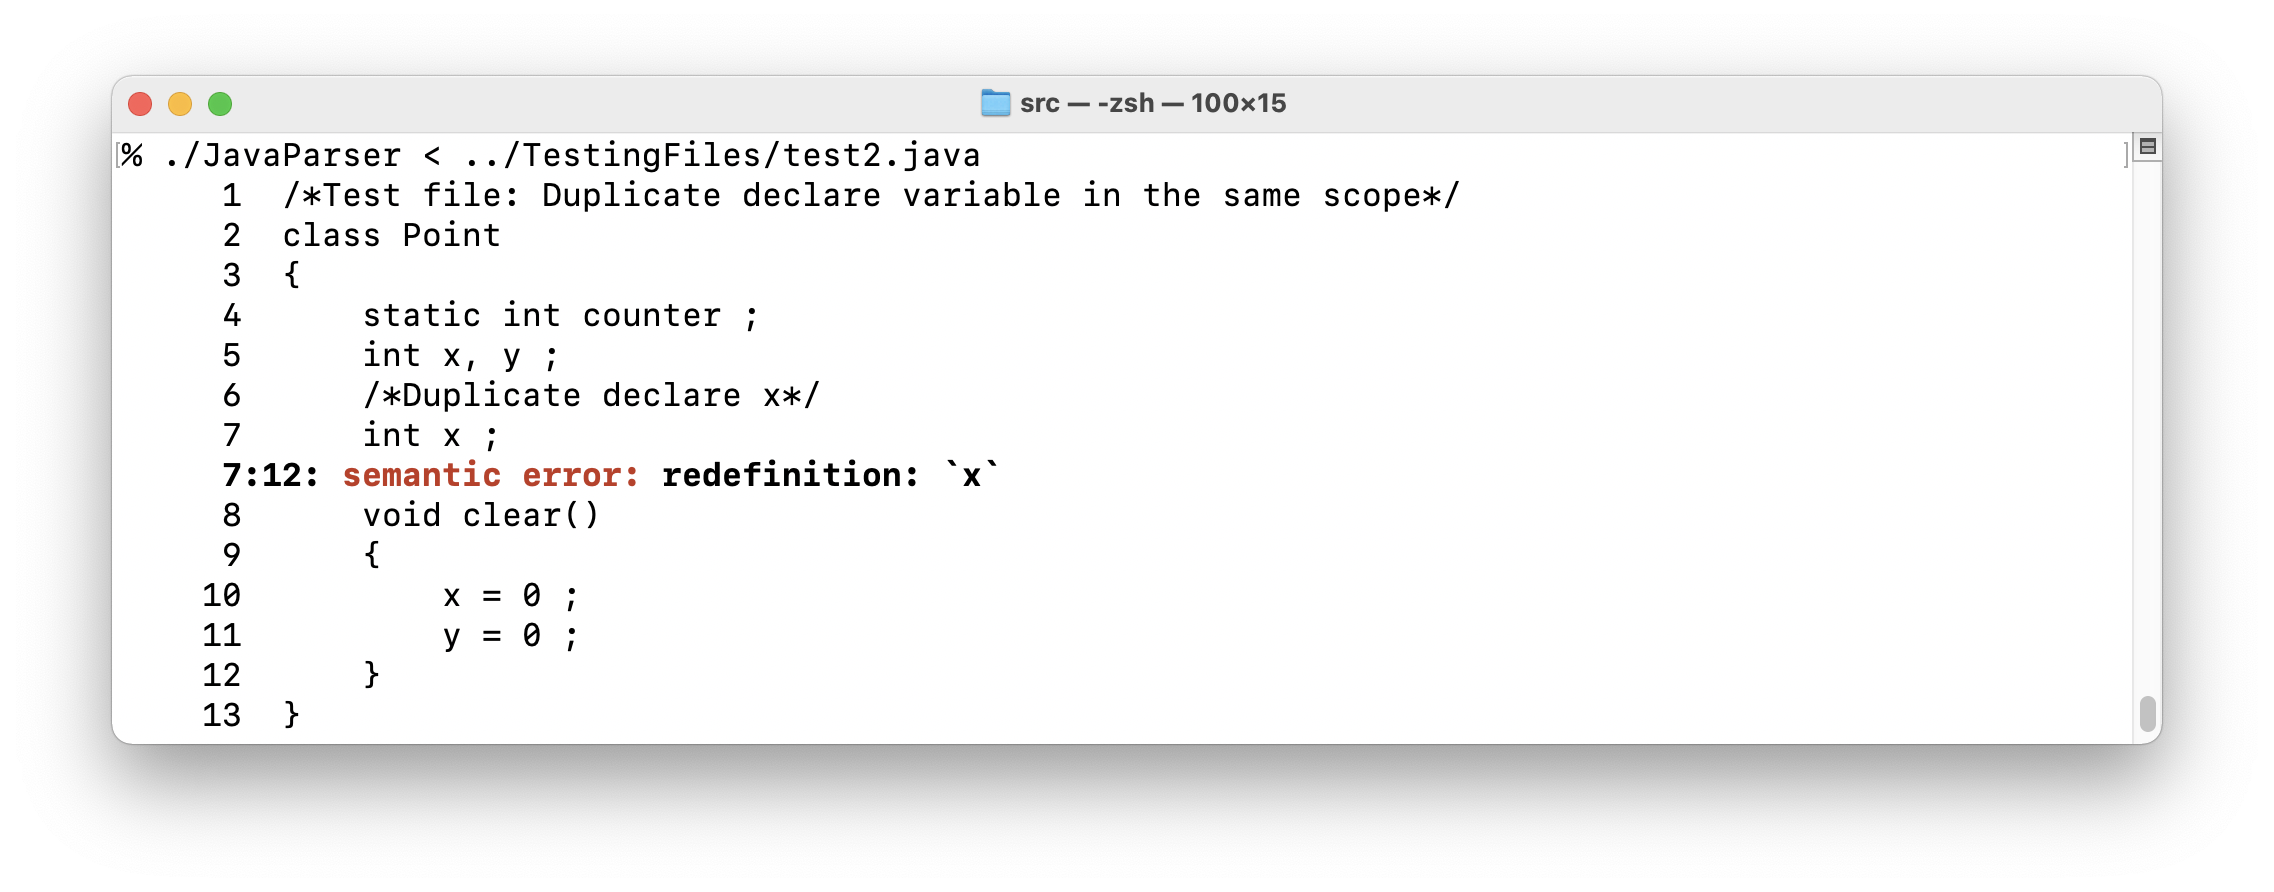
\includegraphics[width=0.9\textwidth]{Screenshots/test2}
\end{center}
\caption{The output of parsing \texttt{test2.java} with \texttt{DEBUG=1}}
\label{test1}
\end{figure}
\begin{figure}
\begin{center}
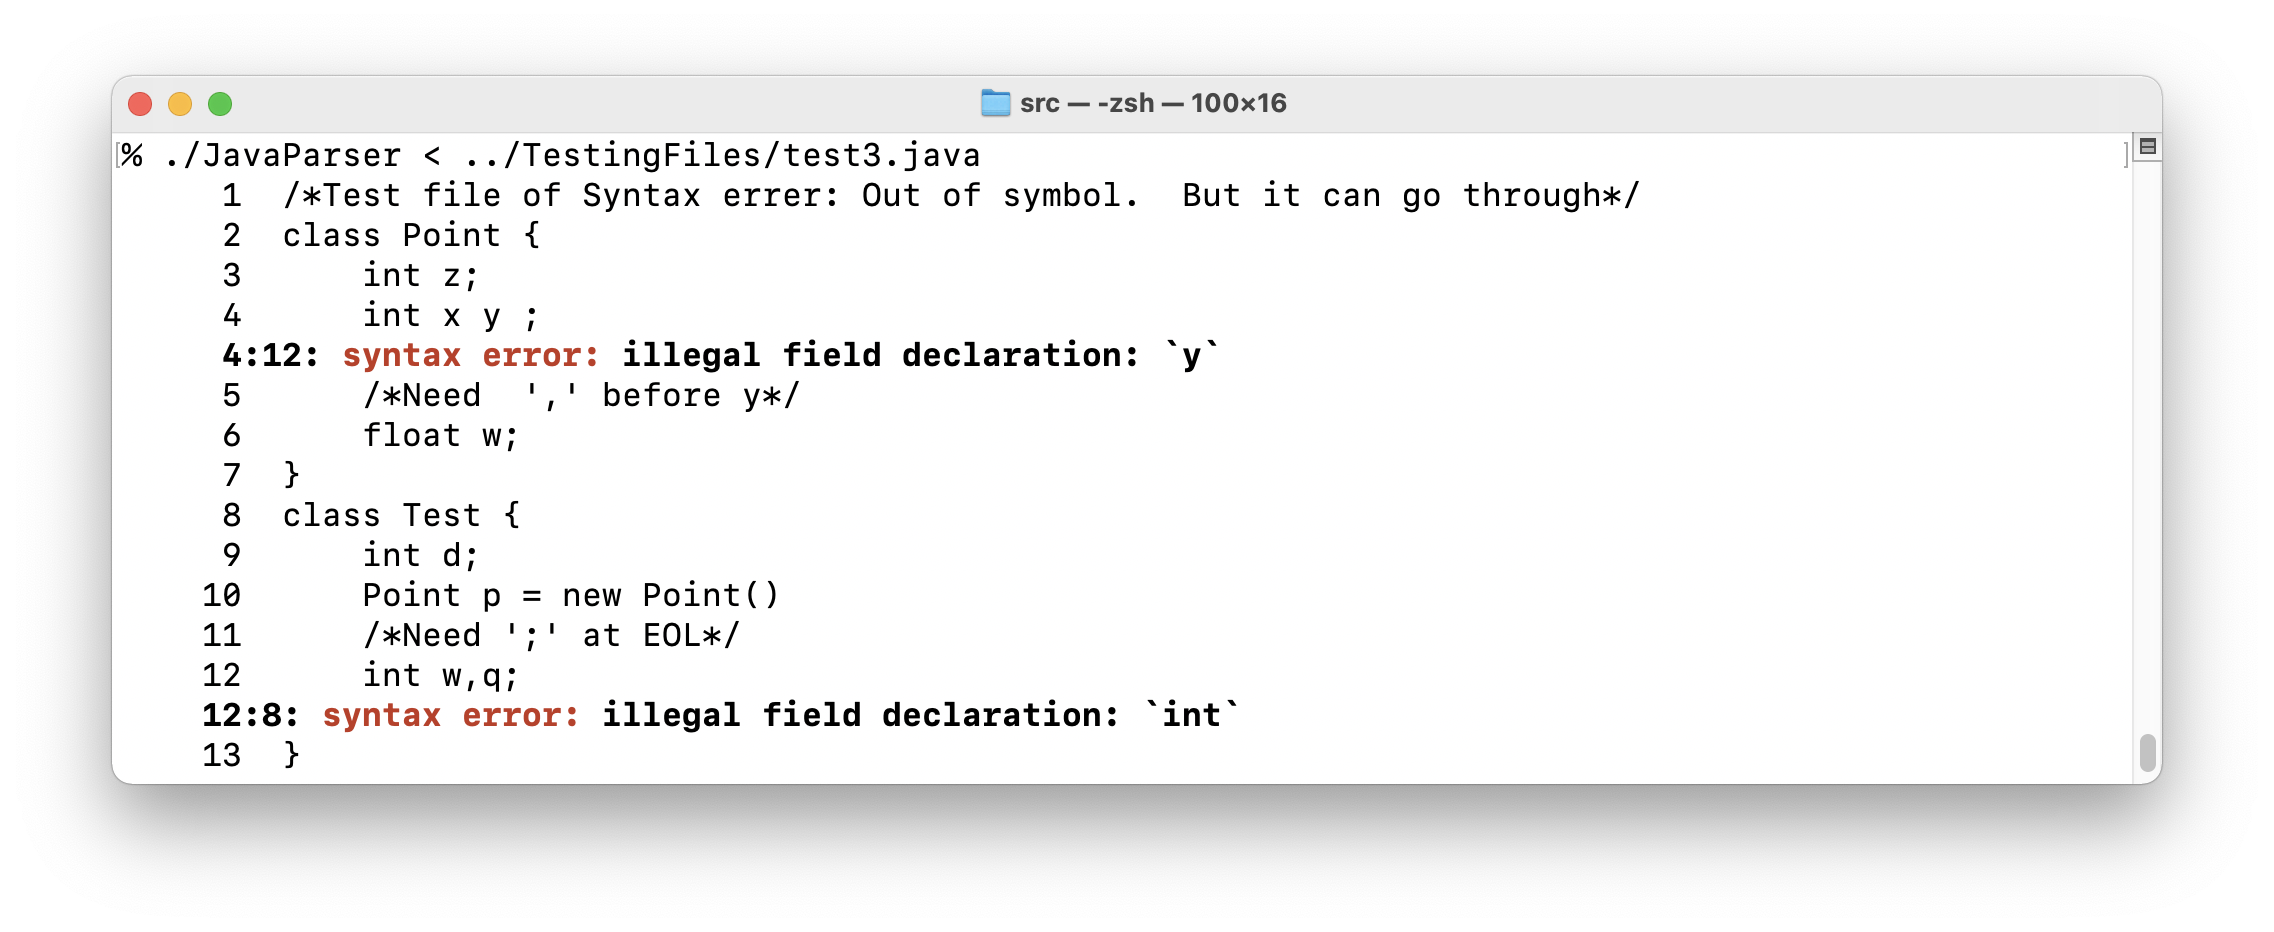
\includegraphics[width=0.9\textwidth]{Screenshots/test3}
\end{center}
\caption{The output of parsing \texttt{test3.java} with \texttt{DEBUG=1}}
\label{test1}
\end{figure}
\begin{figure}
\begin{center}
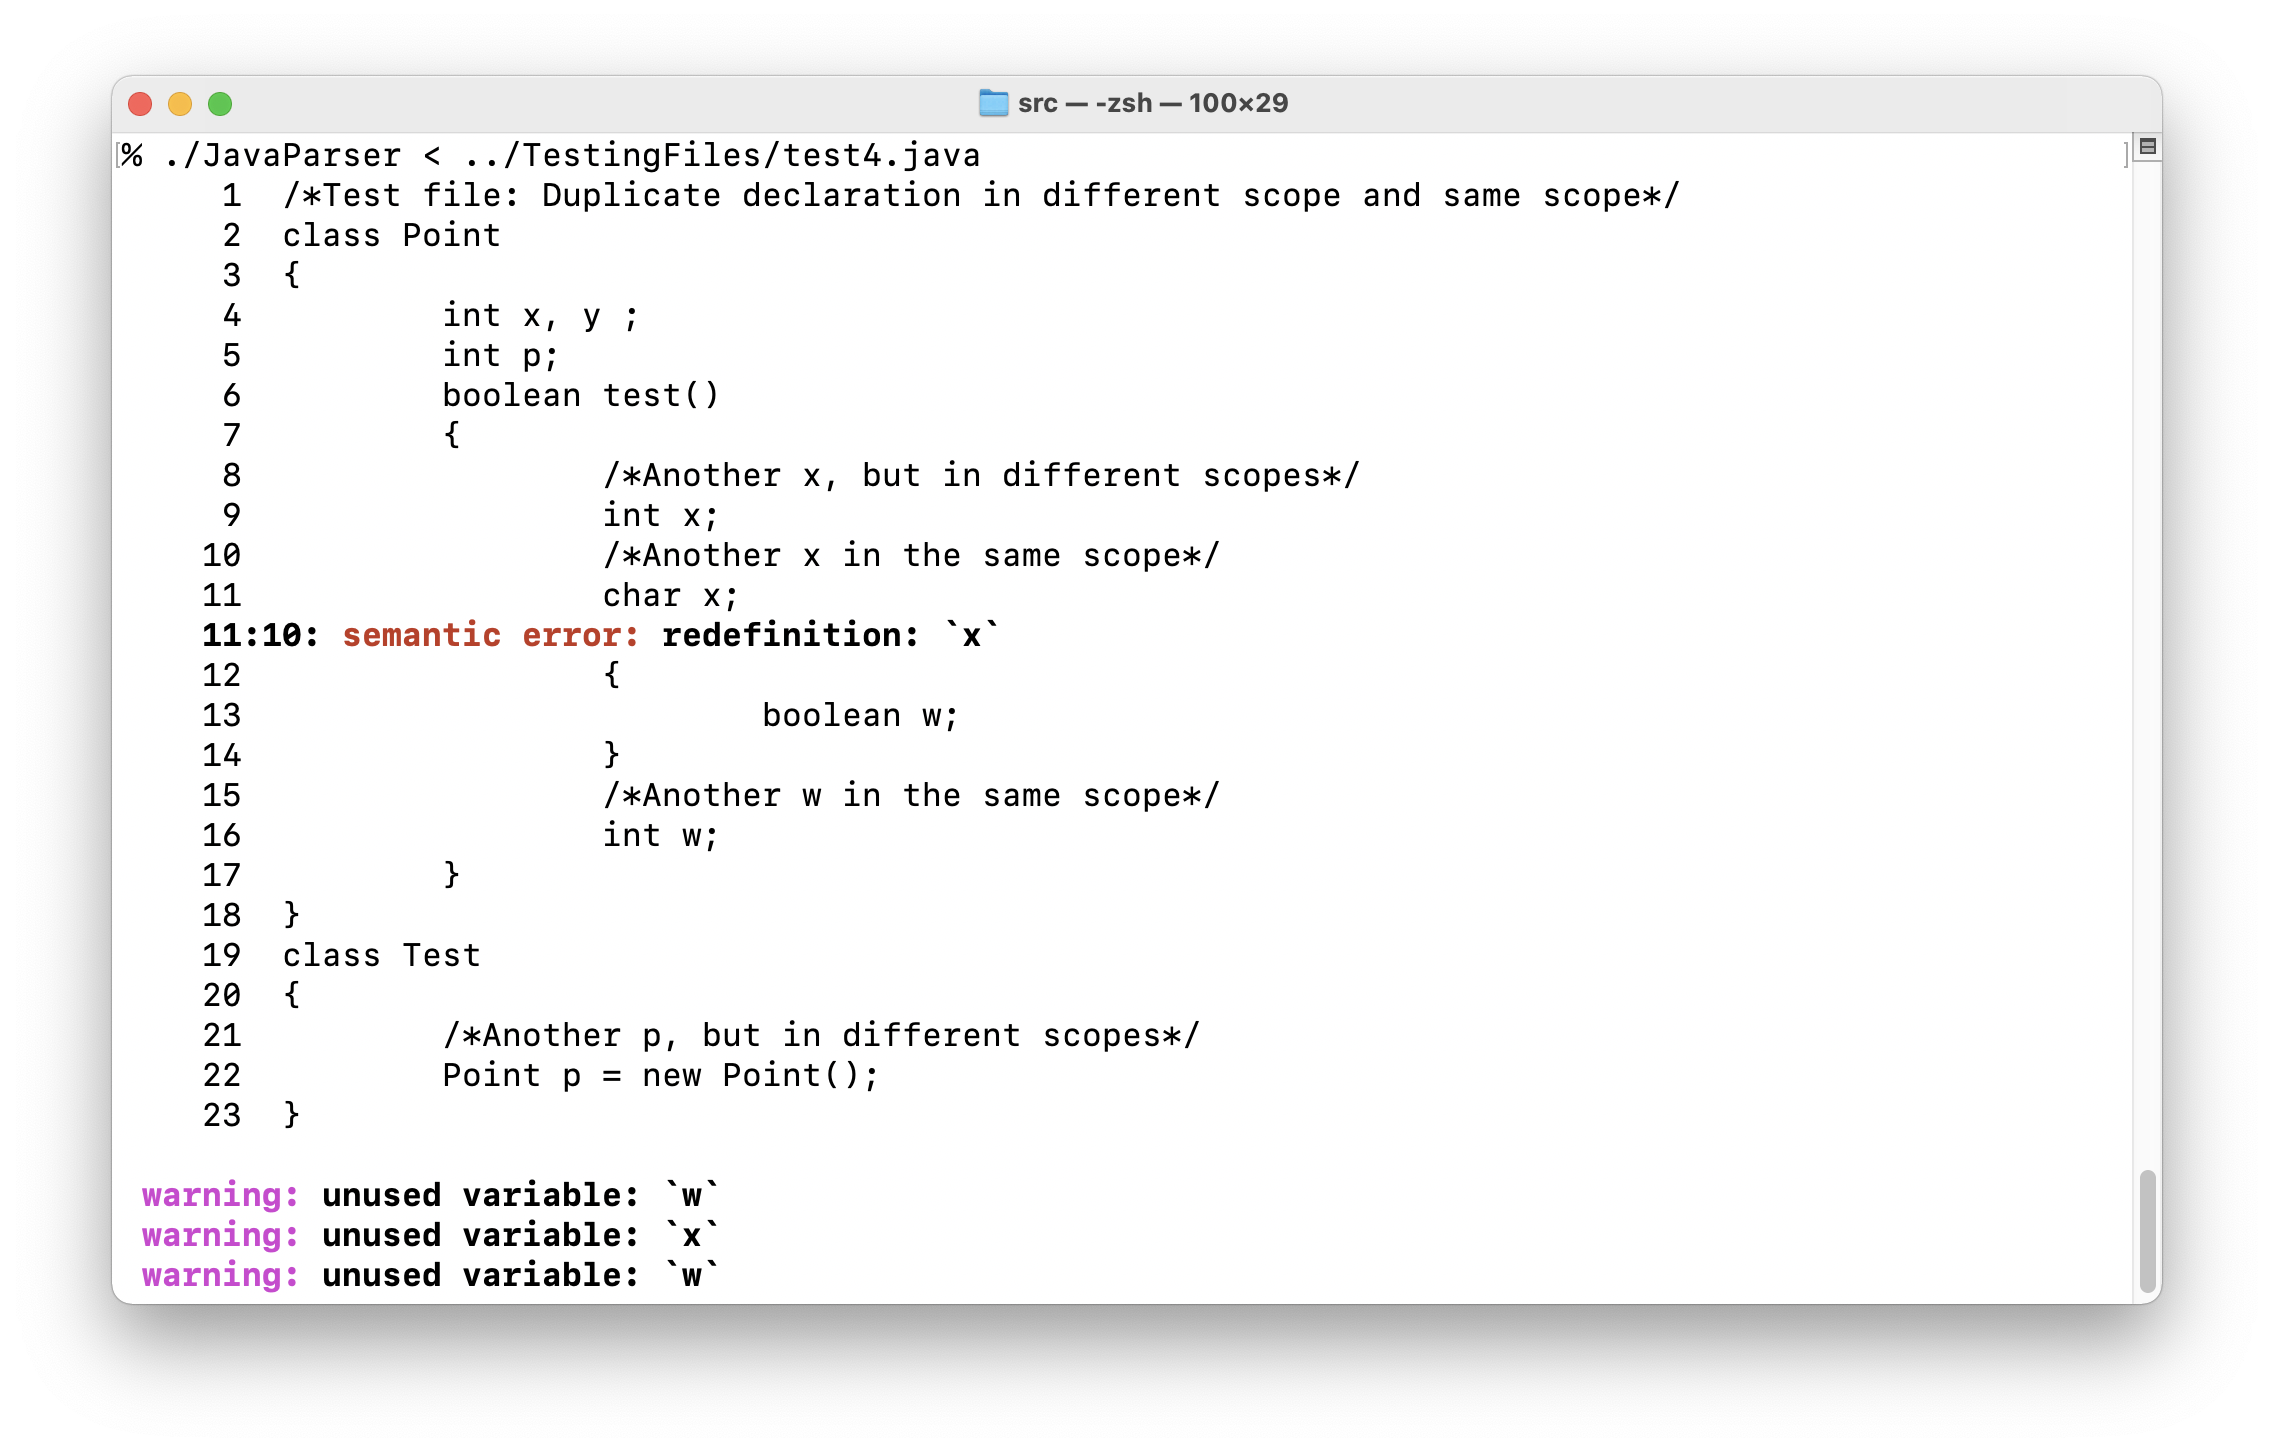
\includegraphics[width=0.9\textwidth]{Screenshots/test4}
\end{center}
\caption{The output of parsing \texttt{test4.java} with \texttt{DEBUG=1}}
\label{test1}
\end{figure}
\begin{figure}
\begin{center}
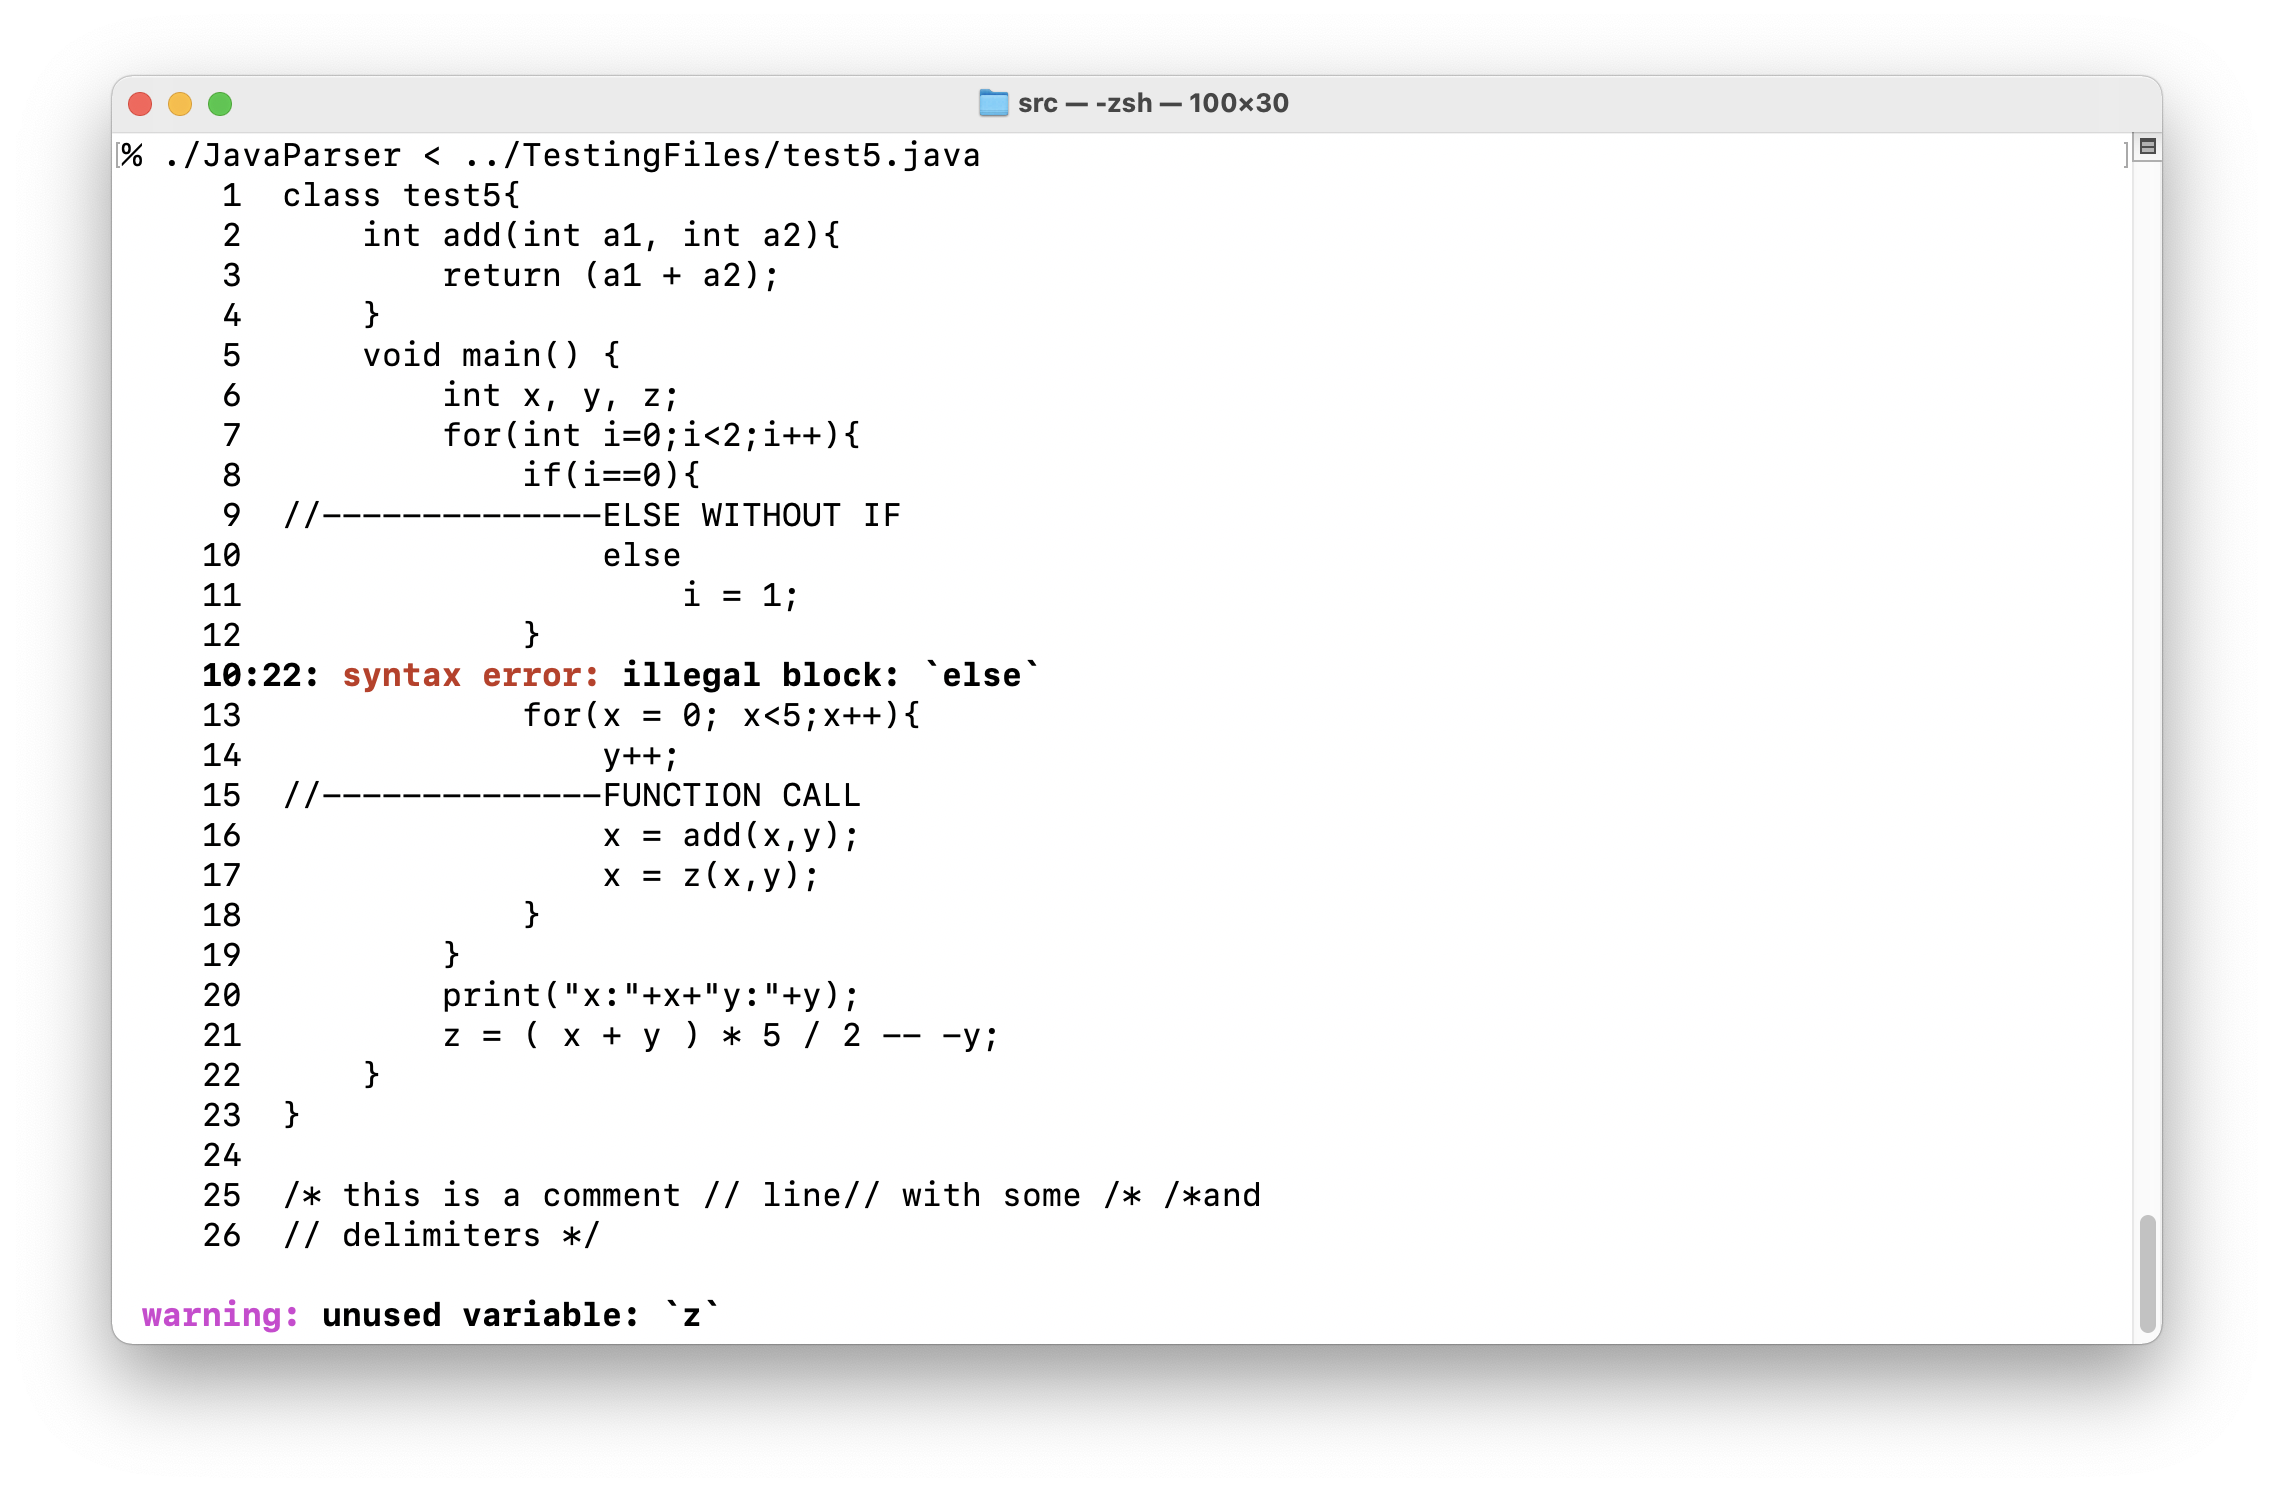
\includegraphics[width=0.9\textwidth]{Screenshots/test5}
\end{center}
\caption{The output of parsing \texttt{test5.java} with \texttt{DEBUG=1}}
\label{test1}
\end{figure}
\begin{figure}
\begin{center}
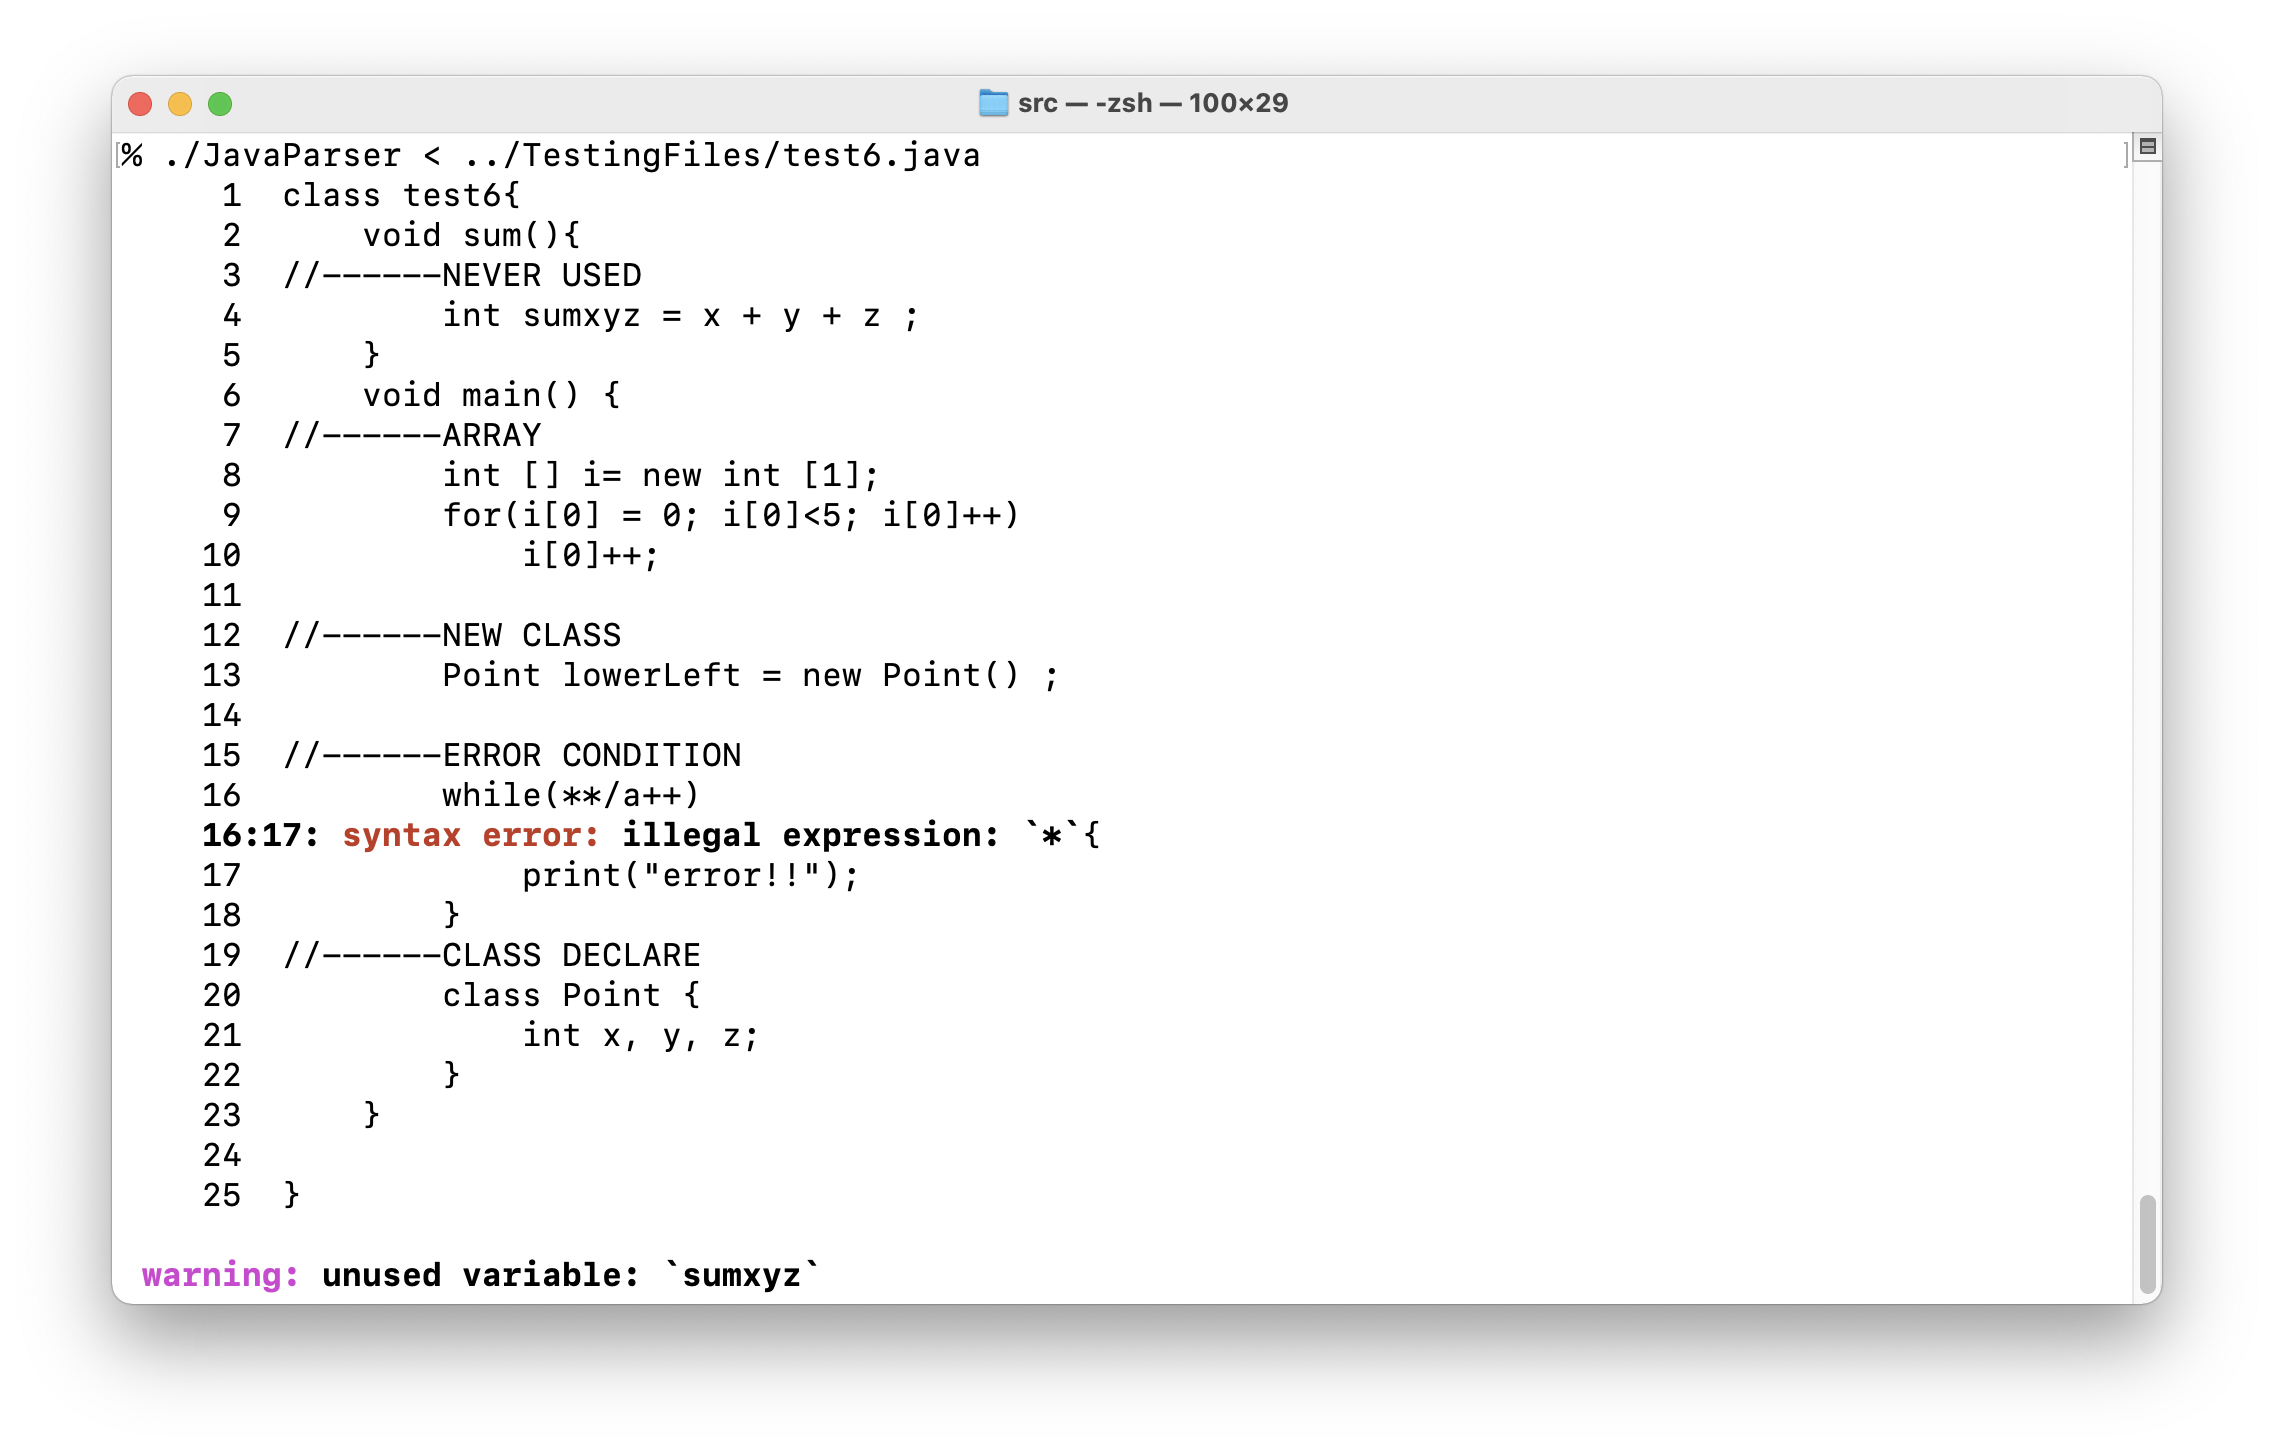
\includegraphics[width=0.9\textwidth]{Screenshots/test6}
\end{center}
\caption{The output of parsing \texttt{test6.java} with \texttt{DEBUG=1}}
\label{test1}
\end{figure}

\newpage
\bibliography{Citations}

\end{document}
